% https://tex.stackexchange.com/a/442718/173708
\PassOptionsToPackage{table,dvipsnames,svgnames}{xcolor}
\documentclass[tikz,margin=1cm]{standalone}
\usetikzlibrary{arrows.meta,calc,positioning}

\colorlet{A}{gray}
\colorlet{B}{lightgray}
\pgfdeclarelayer{background}
\pgfdeclarelayer{timeline}
\pgfdeclarelayer{period}
\pgfdeclarelayer{foreground}
\pgfsetlayers{background,timeline,period,main,foreground}

%https://tex.stackexchange.com/a/349215
\tikzset{
  timeline/.style={arrows={}}%
  ,timeline style/.style={timeline/.append style={#1}}%
  ,year label/.style={font=\Huge\sffamily\bfseries,below}%
  ,year label style/.style={year label/.append style={#1}}%
  ,year tick/.style={tick size=5pt}%
  ,year tick style/.style={year tick/.append style={#1}}%
  ,minor tick/.style={tick size=2pt, very thin}%
  ,minor tick style/.style={minor tick/.append style={#1}}%
  ,period/.style={solid,line width=\timelinewidth,line cap=square}%
  ,periodbox/.style={font=\Huge\sffamily\bfseries,text=black}%
  ,eventline/.style={draw,red,thick,line cap=round,line join=round}%
  ,eventbox/.style={rectangle,rounded corners=3pt,inner sep=3pt,fill=red!25!white,text width=3cm,anchor=west,text=black,align=left,font=\large}%
  ,tick size/.code={\def\ticksize{#1}}%
  ,labeled years step/.code={\def\yearlabelstep{#1}}%
  ,minor tick step/.code={\def\minortickstep{#1}}%
  ,year tick step/.code={\def\yeartickstep{#1}}%
  ,enlarge timeline/.code={\def\enlarge{#1}}%
  ,eventboxa/.style={eventbox,text width=#1,draw=A,fill=none}%
  ,eventboxb/.style={eventbox,text width=#1,draw=A,fill=none}%
}

% Still from %https://tex.stackexchange.com/a/349215
\newcommand*{\drawtimeline}[5][]{%
  \def\fromyear{#2}%
  \def\toyear{#3}%
  \def\timelinesize{#4}%
  \def\timelinewidth{#5}%
  \pgfmathsetmacro{\timelinesizept}{\timelinesize}%
  \pgfmathsetmacro{\timelinewidthpt}{\timelinewidth}%
  \pgfmathsetmacro{\timelineoffset}{\timelinewidth/2}
  \pgfmathsetmacro{\timelineoffsetpt}{\timelineoffset}
%
  \begin{scope}[x=1pt, y=1pt, % Change main units to pt
                labeled years step=1,% Set some defaults
                minor tick step=0.25,%
                enlarge timeline=0cm,%
                year tick step=1,#1]
    \pgfmathsetmacro{\enlargept}{\enlarge}
    \pgfmathsetmacro{\yearticksep}{\timelinesize/((\toyear-\fromyear)/\yeartickstep)}
    \pgfmathsetmacro{\minorticksep}{\timelinesize/((\toyear-\fromyear)/\minortickstep)}
    \pgfmathsetmacro{\minorticklast}{\minorticksep/\minortickstep}
    \foreach \y[remember=\y as \lasty (initially 0), count=\i from \fromyear] in {0,\yearticksep,...,\timelinesizept}{
        \coordinate (Y-\i) at (\y,0);
        \draw[year tick] (\y,-\ticksize/2) --  ++(0,\ticksize);
        \ifnum\i=\toyear\breakforeach\else
        \foreach \q[count=\j from 0] in {0,\minorticksep,...,\minorticklast}{
            \coordinate (Y-\i-\j) at (\q+\y,0);
                \begin{pgfonlayer}{timeline}
            \draw[minor tick] (\q+\y,-\ticksize/2) -- ++(0,\ticksize);
                \end{pgfonlayer}
        };\fi};%
    \pgfmathsetmacro{\nextyear}{int(\fromyear+\yearlabelstep)}
    \begin{pgfonlayer}{timeline}
    \draw[timeline] (0,0) -- ++(-\enlargept,0) (0,0) -- ++(\timelinesizept,0) coordinate (end) -- ++(\enlargept,0);% Timeline
    \end{pgfonlayer}
%    \foreach \y in {\fromyear,\nextyear,...,\toyear} \node[year label] at (Y-\y) {\y};
  \end{scope}%
}
% Put a period identifier midway between the start and end of the period
% 1 = color of timeline segment
% 2 = period start
% 3 = period end
% 4 = period text
\newcommand{\period}[5]{\begin{pgfonlayer}{period} \draw[period,#1] (Y-#2) -- (Y-#3) node[periodbox,#5,midway,text=white] {\begin{tabular}{l} #4 \end{tabular}}; \end{pgfonlayer}}

%This somewhat follows @cfr's Chronos. It was certainly inspired by Chronos.
%https://tex.stackexchange.com/a/349236

% 1 = format of line and box
% 2 = starting coordinate
% 3 = pin associated with starting coordinate (well suited to using polar coordinate)
% 4 = branch at top of pin (well suited to using polar coordinate)
% 5 = Any extra formatting of node
% 6 = Name of node
% 7 = Node content

\newcommand{\vevent}[7]{\begin{pgfonlayer}{timeline} \draw[eventline,#1](Y-#2) -- ++(#3) -- ++(#4) node[#5] (#6) {#7}; \end{pgfonlayer}}

\begin{document}
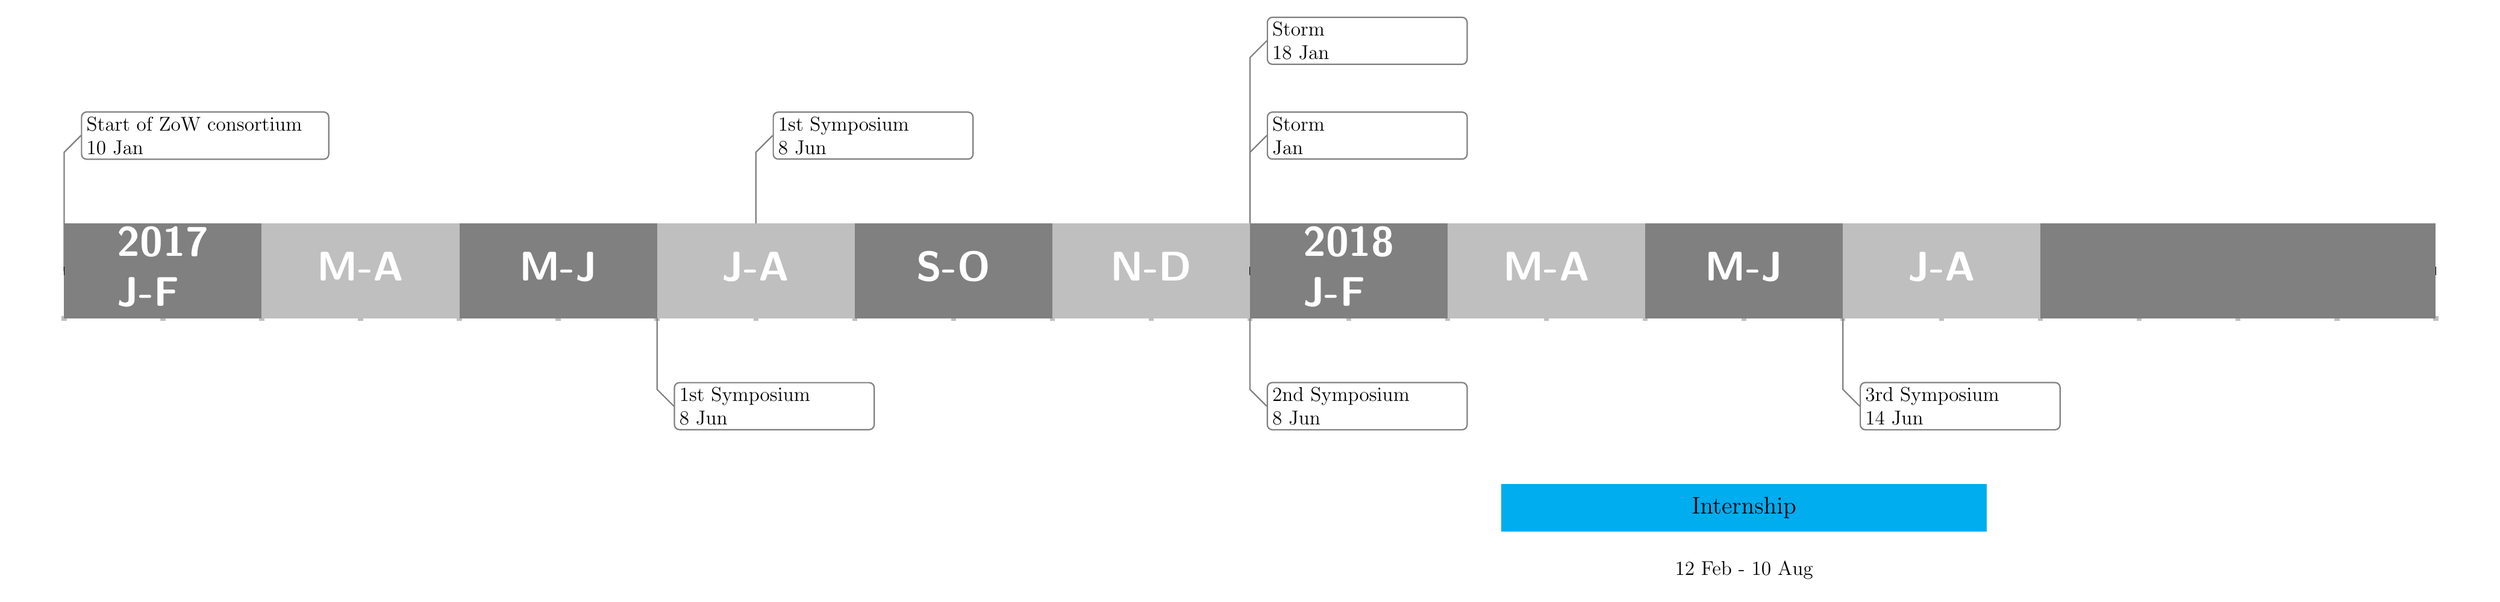
\begin{tikzpicture}
    \drawtimeline[
        labeled years step=1,
        minor tick step=0.083333,
        timeline style={draw=gray,line width=\timelinewidthpt},
        minor tick style={-,lightgray,tick size=3pt,line width=3pt,yshift=-\timelineoffsetpt},           
        ]%
        {2017}{2019}{50cm}{2cm};
    %
    \period{A}{2017-0}{2017-2}{2017\\J-F}{}
    \period{B}{2017-2}{2017-4}{M-A}{}
    \period{A}{2017-4}{2017-6}{M-J}{}
    \period{B}{2017-6}{2017-8}{J-A}{}
    \period{A}{2017-8}{2017-10}{S-O}{}
    \period{B}{2017-10}{2017-12}{N-D}{}
    \period{A}{2018-0}{2018-2}{2018\\J-F}{}
    \period{B}{2018-2}{2018-4}{M-A}{}
    \period{A}{2018-4}{2018-6}{M-J}{}
    \period{B}{2018-6}{2018-8}{J-A}{}
    %
    \vevent{A}{2017-0}{90:2.5cm}{45:0.5cm}{eventboxa=5cm,anchor=west}{H}{Start of ZoW consortium\\10 Jan}
    \vevent{A}{2017-6}{-90:2.5cm}{-45:0.5cm}{eventboxa=4cm,anchor=west}{H}{1st Symposium\\8 Jun}    
    \vevent{A}{2017-7}{90:2.5cm}{45:0.5cm}{eventboxa=4cm,anchor=west}{H}{1st Symposium\\8 Jun} 
    \vevent{A}{2017-12}{-90:2.5cm}{-45:0.5cm}{eventboxa=4cm,anchor=west}{H}{2nd Symposium\\8 Jun} 
    \vevent{A}{2018-0}{90:2.5cm}{45:0.5cm}{eventboxa=4cm,anchor=west}{H}{Storm\\Jan} 
    \vevent{A}{2018-0}{90:4.5cm}{45:0.5cm}{eventboxa=4cm,anchor=west}{H}{Storm\\18 Jan} 
    \vevent{A}{2018-6}{-90:2.5cm}{-45:0.5cm}{eventboxa=4cm,anchor=west}{H}{3rd Symposium\\14 Jun}
    %
    \node[draw=none,rectangle,fill=cyan,text width=10cm,minimum height=1cm,text=black,align=center,font=\Large] (AA) at  ([yshift=-5cm]Y-2018-5) {Internship};       
    \node[below=0.5cm of AA,font=\large] {12 Feb - 10 Aug};            
\end{tikzpicture}
\end{document}